\documentclass[11pt,a4paper]{article}

\usepackage{geometry}
 \geometry{
 a4paper,
 total={150mm,237mm},
 left=30mm,
 top=30mm,
 }

% cf. http://tex.stackexchange.com/questions/50182/subtitle-with-the-maketitle-page
\usepackage{titling}
\newcommand{\subtitle}[1]{%
  \posttitle{%
    \par\end{center}
    \begin{center}\large\textbf{#1}\end{center}
    \vskip0.5em}%
}

\usepackage{color}
\usepackage{graphicx}
\usepackage{subcaption}

\usepackage[utf8]{inputenc}
\usepackage[lf]{venturis} %% lf option gives lining figures as default; 
\usepackage[T1]{fontenc}
\usepackage{beramono}
\usepackage{csquotes}
\usepackage[UKenglish,german]{babel}

\usepackage{fancyvrb}

\widowpenalty10000  % http://tex.stackexchange.com/questions/4152/how-do-i-prevent-widow-orphan-lines
\clubpenalty10000

\title{The SysSon Platform}
\subtitle{Technical Report TR-2016-10-1\\Institute of Electronic Music and Acoustics, Graz\\(Status: in progress)}
\author{Hanns Holger Rutz}
% \date{09-Feb-2016}
\date{October 2016}

% cf. https://tex.stackexchange.com/questions/94126/change-font-to-only-section-and-subsection-of-my-document
%\usepackage{titlesec}
%\titleformat{\chapter}[display]
%  {\fontfamily{pag}\selectfont\huge\bfseries}
%  {\chaptertitlename\ \thechapter}
%  {20pt}
%  {\Huge}
%\titleformat{\section}
%  {\fontfamily{pag}\selectfont\bfseries\Large}
%  {\thesection}
%  {1em}
%  {}
%\titleformat{\subsection}
%  {\fontfamily{pag}\selectfont\bfseries\Large}
%  {\thesection}
%  {1em}
%  {}

\usepackage[backend=biber,authordate]{biblatex-chicago} % citereset=chapter
%\usepackage[backend=biber,natbib,isbn=false,useprefix=true,sorting=ydnt]{biblatex-chicago} % citereset=chapter
\addbibresource{all.bib} % add a bib-reference file
\addbibresource{rutz.bib} % add a bib-reference file

% warning: https://tex.stackexchange.com/questions/313477/
% \usepackage{csquotes}

\usepackage{tabularx}
% cf. https://tex.stackexchange.com/questions/84400/table-layout-with-tabularx-column-widths-502525
\newcolumntype{s}{>{\hsize=1cm}X}

% says you should load after babel and fontspec
\usepackage[shrink=10, babel=true]{microtype}	% http://tex.stackexchange.com/questions/141852/latex-allows-line-break-between-concluding-em-dash-and-comma-before-a-new-sub-cl/141854#141854

% has to come first for full scale TeX voodoo bullcrap
\usepackage{hyperref}
% get rid of the horrible coloured boxes around links
\hypersetup{
    colorlinks,%
    citecolor=black,%
    filecolor=black,%
    linkcolor=black,%
    urlcolor=black
}
% has to come after frickin hyperref
\VerbatimFootnotes

\newcommand{\todo}[1]{\colorbox{yellow}{\textsc{todo}: #1}}

\newcommand{\quot}[1]{\guillemotleft {#1}\guillemotright}

\newcommand{\worktitle}[1]{\textit{#1}}

\newcommand{\workentry}[2]{\vspace{7.5pt}\noindent\textbf{#1} (#2)}
\newcommand{\workentrySel}[2]{\vspace{7.5pt}\noindent\textbf{#1}$*$ (#2)}

\newcommand{\figref}[1]{Fig.~\ref{#1}}

\newcommand{\software}[1]{\textit{#1}}

\newcommand{\sysson}[0]{SysSon}
\newcommand{\syssonVersion}[0]{1.8.0}
\newcommand{\syssonVersionS}[0]{1.8.0-SNAPSHOT}

\newcommand{\artefacts}[0]{\textsc{Artefacts:}}
\newcommand{\assessment}[0]{\textsc{Assessment:}}

\usepackage{listings}

\definecolor{dkgreen}{rgb}{0,0.6,0}
\definecolor{gray}{rgb}{0.5,0.5,0.5}
\definecolor{mauve}{rgb}{0.58,0,0.82}

\lstdefinestyle{plain}{
  frame=tb,
  aboveskip=3mm,
  belowskip=3mm,
  showstringspaces=true,
  columns=flexible,
  basicstyle={\small\ttfamily},
  numbers=none,
  numberstyle=\tiny\color{gray},
  keywordstyle=\color{blue},
  commentstyle=\color{dkgreen},
  stringstyle=\color{mauve},
  frame=none,
  keepspaces=true,
  breaklines=true,
  breakatwhitespace=true,
  tabsize=3,
}

\lstdefinestyle{scala}{
  frame=tb,
  language=scala,
  aboveskip=3mm,
  belowskip=3mm,
  showstringspaces=true,
  columns=flexible,
  basicstyle={\small\ttfamily},
  numbers=none,
  numberstyle=\tiny\color{gray},
  keywordstyle=\color{blue},
  commentstyle=\color{dkgreen},
  stringstyle=\color{mauve},
  frame=none,
  keepspaces=true,
  breaklines=true,
  breakatwhitespace=true,
  tabsize=3,
}

\lstdefinestyle{scala-small}{
  frame=tb,
  language=scala,
  aboveskip=3mm,
  belowskip=3mm,
  showstringspaces=true,
  columns=flexible,
  basicstyle={\tiny\ttfamily},
  numbers=none,
  numberstyle=\tiny\color{gray},
  keywordstyle=\color{blue},
  commentstyle=\color{dkgreen},
  stringstyle=\color{mauve},
  frame=none,
  keepspaces=true,
  breaklines=true,
  breakatwhitespace=true,
  tabsize=3,
}

\begin{document}
% \begin{titlepage}
\maketitle
\selectlanguage{UKenglish}
\thispagestyle{empty}
\newpage
\section{First Sonification Scenario}

Following a project meeting on 16-Sep-2016, it was decided that the first scenario or template to work out is to look at QBO (quasi-biennial-oscillation) and ENSI (El Niño), using two sets of measured temperature data.\footnote{%
A different scenario discussed are "stratospheric sudden warmings", which happen around the poles in 30\,km altitude. The sudden jumps in temperature of up to 70 degrees happen within  weeks, and proceed from top to bottom.%
}

We had worked with QBO sonification already in one of the previous workshops. One usually selects a specific range in the altitudes and rather equatorial coordinates (e.g. +/- 10 degrees). Longitudes are often averaged, but we will try to also look at longitudinal movements.

QBO and ENSO interact with each other in that strong amplitudes in ENSO (lower altitudes) are connected with the inverse phenomena in the QBO (higher altitudes). It would thus be interesting to be also able to sonically compare the two.

\subsection{Data Files}

\begin{itemize}
\item {\small \Verb!5x5-climatology_2001-05-01_2016-05-01_RO_OPSv5.6.2_L2b_no_METOP_no_TerraSAR-X.nc!}\\A high-resolution file with 5x5 latitude/longitude grid, 600 altitude levels, and over 180 months (10.1\,GB)
\item {\small \Verb!5x30-climatology_2001-05-01_2016-05-01_RO_OPSv5.6.2_L2b_no_METOP_no_TerraSAR-X.nc!}\\A slightly lower resolution file with 5x50 latitude/longitude grid (1.7\,GB)
\end{itemize}

Initial problems:
%
\begin{itemize}
\item File selection filter did not know about HDF files (previously only NetCDF files were used); \textbf{Result: fixed}
\item Heatmap plots somehow fail to gather the statistics of the data. \textbf{Result: It is just running very slowly (c. 12 minutes).}
\item After stats finally complete, data is useless because we don't have fill value information, and apparently something different from NaN is used. \textbf{Result: Converted file to use NaNs}
\item Date format not recognised. Time unit is "seconds since 1990-01-01T00:00:00", somehow that is not correctly parsed. \textbf{Result:  fixed}
\item The dimensions "Latitude" and "Longitude" are not correctly recognised, because the map-overlay option is not shown. \textbf{Result: fixed}
\end{itemize}
%
We might:
%
\begin{itemize}
\item look into updating the NetCDF library and drop Java 6 support. New artifact is called \Verb!netcdf4! and latest version is 4.6.6. This might improve performance. \textbf{Result: no speed improvement}
\item introduce a simple table view, so one can quickly browse the data numerically.
\item create a preference item to \emph{disable} automatic removal of cache upon application quit.
\item we also need to be able to adjust the cache size, because the 1.7 GB files produces already a 230 KB stats cache, therefore we will easily transcend the default cache size of 1 MB.
\end{itemize}
%
After further inspection, fill values are correctly stored and found as -1e-10. Strangely stats show a max of 2.4e22 and a mean of 5.1e14. For example, for dry temperature those values appear in time index 90 and altitude indices 5 to 8. Here a "spike" of 4.49e23 in altitude index 5 declines towards index 8, and at index 9 the data is in the normal range again. We thus need to first preprocess that file and replace out-of-range values with the defined fill value. \textbf{Result: fixed by converting data.}

Intuition was, that because of possibly more slight glitches in the data, using the median instead of the mean for the calculation of anomalies might be better or more robust. We added this option to the anomaly utility of \software{SysSon}. \figref{fig:anomaly-calc} shows the difference between these two variants. It can be observed that using the mean monthly value as a basis results in a smoother plot, whereas using the median gives more pronounced deviations. Overall, the differences are small, though, and probably will not lead to significantly different sounds.

\begin{figure}
% \centering
\begin{subfigure}[b]{1.0\textwidth}%
\centering
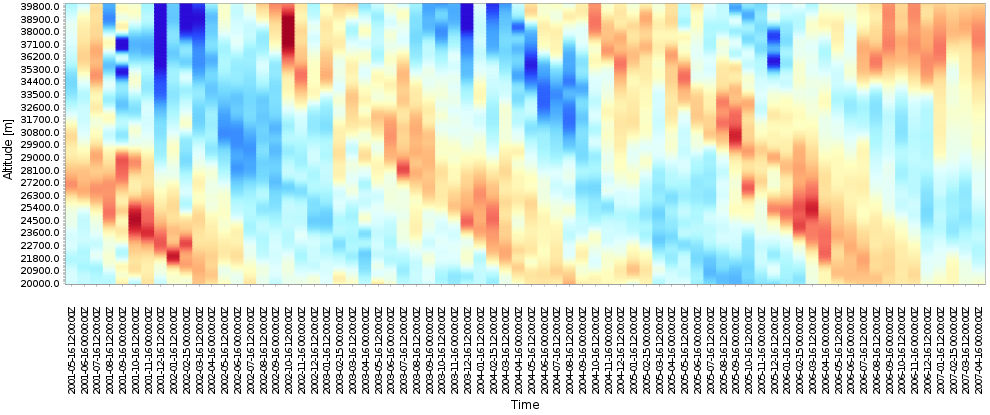
\includegraphics[scale=0.45,trim=2mm 0 1mm 1mm]{figures/ta_anomalies_mean.jpg}
\caption{Using monthly mean}
\label{fig:anomaly-mean}
\end{subfigure}
\begin{subfigure}[b]{1.0\textwidth}%
\centering
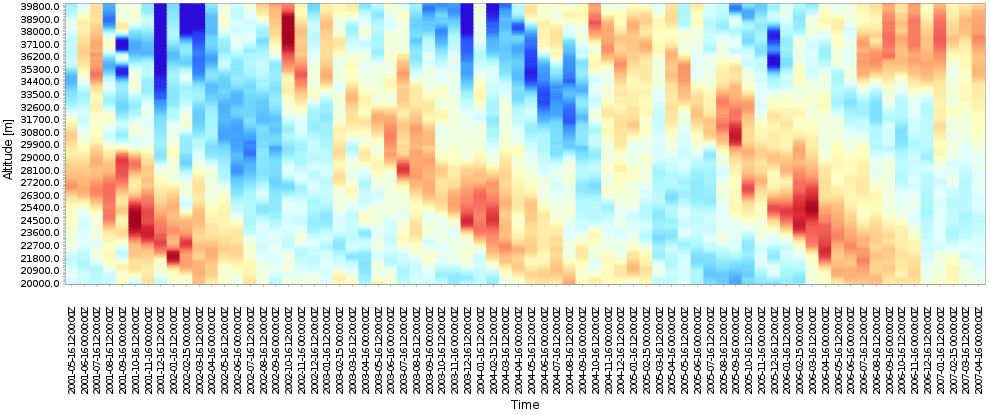
\includegraphics[scale=0.45,trim=2mm 0 1mm -4mm]{figures/ta_anomalies_median.jpg}
\caption{Using monthly median}
\label{fig:anomaly-median}
\end{subfigure}
\caption{Temperature anomalies calculated with different norms. Indices where taken at longitude 105 degrees west, and latitude 2.5 degrees south. The expected periodicity of 28 to 29 months can be clearly seen.}
\label{fig:anomaly-calc}
\end{figure}

\subsection{First Sound Models}

In the first model, time in the dataset is simply mapped to time in the sonification. We use a longitude and latitude index, and a slice of the altitudes, similar to the selection made in \figref{fig:anomaly-calc}.

Questions:
%
\begin{itemize}
\item How do we ``connect trajectories'' and avoid steps (in time, because the altitude has a fine resolution)?
\item How do we distinguish too-cold and too-hot? We could in any case project them onto left and right channel, respectively.
\item Altitude resolution is high, we select roughly 200 bands.
\end{itemize}
%

The code for the first sketch is shown in \figref{fig:sketch-1}. There is a simple threshold \Verb!vp > 1! that selects only the too-hot anomalies. Each altitude where this filter applies is represented by a sine oscillator with a frequency corresponding to the altitude (logarithmically scaled from 200 Hz to 4 kHz across the selected altitudes).

\begin{figure}
\begin{lstlisting}[style=scala]
val vr     = Var("anom")
val dTime  = Dim(vr, "time")
val dAlt   = Dim(vr, "altitude")

val speed  = UserValue("speed", 1).kr
val tp     = dTime.play(speed)
val vp     = vr.play(tp, interp = 2)

val hot    = vp > 1
val amp    = hot * (vp.min(8) / 8)
val alt    = vp.axis(dAlt).values
val altMin = Reduce.min(alt)
val altMax = Reduce.max(alt)

val freq   = alt.linexp(altMin, altMax, 200, 4000)
val sin    = Mix.mono(SinOsc.ar(freq) * amp) / dAlt.size

output := Pan2.ar(sin)
\end{lstlisting}
\caption{First sketch; filtering only high temperatures,
mapping them each to an oscillator.}
\label{fig:sketch-1}
\end{figure}

The sonic result is a dense texture with a metallic timbre. Not much details can be distinguished, but the overall downward glissando is clearly heard. One can also here some irregularities in the movement.

Looking again at the visual plot, it seems useful to reduce the amount of oscillators to capture only the significant properties, such as following the peak of the temperature profile. Without further offline pre-processing, the third-party UGen \Verb!ArrayMax! is a useful building block for detecting the global maximum in a multi-channel signal. In \figref{fig:sketch-2} this is used to produce the frequency of a single oscillator.

\begin{figure}
\begin{lstlisting}[style=scala]
val vr    = Var("anom")
val dTime = Dim(vr, "time")
val dAlt  = Dim(vr, "altitude")

val speed = UserValue("speed", 1).kr
val tp    = dTime.play(speed)
val vp    = vr.play(tp, interp = 1)

val max   = ArrayMax.ar(vp)
val freq0 = max.index.linexp(0, dAlt.size - 1, 200, 4000)
val freq  = Ramp.ar(freq0, 1.0/speed)
val amp0  = max.value.clip(0, 8) / 8
val amp   = Ramp.ar(amp0, 1.0/speed)
val sin   = SinOsc.ar(freq) * amp

output := Seq(DC.ar(0), sin)
\end{lstlisting}
\caption{Second sketch; reducing to one oscillator at maximum bin.}
\label{fig:sketch-2}
\end{figure}

This works principally fine, however there are time slices where the global maximum jumps randomly between two local maxima. The next refinement thus would be to distinguish multiple trajectories and try to keep track of their respective frequencies such that jumps are avoided. A number of local maxima can be calculated, if \Verb!ArrayMax! is applied multiple times to a recursively filtered signal, in each iteration subtracting the last detected peak. This idea is illustrated in \figref{fig:sonif-multi-max}.

\begin{figure}
\begin{lstlisting}[style=scala]
...
val max       = ArrayMax.ar(vp)
val maxIdx    = max.index
val numAlt    = dAlt.size
val maskWidth = numAlt / 4
val mask      = vp * ChannelIndices(vp).absdif(maxIdx) > maskWidth
val max2      = ArrayMax.ar(mask)
val maxIdx2   = max2.index
val freq0     = maxIdx.linexp(0, numAlt - 1, 200, 4000)
val freq      = Ramp.ar(freq0, 1.0/speed)
val amp0      = max.value.clip(0, 8) / 8
val amp       = Ramp.ar(amp0, 1.0/speed)
val sin       = SinOsc.ar(freq) * amp

val freq02    = maxIdx2.linexp(0, numAlt - 1, 200, 4000)
val freq2     = Ramp.ar(freq02, 1.0/speed)
val amp02     = max2.value.clip(0, 8) / 8
val amp2      = Ramp.ar(amp02, 1.0/speed)
val sin2      = SinOsc.ar(freq2) * amp2
...
\end{lstlisting}
\caption{Using masking to find multiple ``maxima''}
\label{fig:sonif-multi-max}
\end{figure}

\subsection{Managing Voices and Trajectories}

In order to manage multiple voices on the server side within one synth definition, the idea is to maintain a state matrix. Each row in the matrix corresponds to a ``pre-allocated'' voice. In order to allow voices to decay with an envelope when the trajectory ends, we need more voices than trajectories. A first approximation would be to allocate twice as many voices as the maximum number of expected trajectories. With the QBO data, we probably will want to track not more than four trajectories per polarity (e.g. two to four for the too-hot data, and two to four for the too-cold data). The matrix columns then carry the state of each voice:
%
\begin{itemize}
\item Whether it is currently enabled (``on-off'').
\item The last set frequency or trajectory magnitude
\item The last set amplitude or trajectory strength
\end{itemize}
%
Without writing custom UGens, SuperCollider provides the UGens \Verb!LocalIn! and \Verb!LocalOut! to ``store'' state in a synthesis process. At the beginning of the graph, the previous state is read via \Verb!LocalIn!, at the end of the graph the updated state is written via \Verb!LocalOut!. This feedback mechanism incurs the costs of one control block latency for updated state data to appear earlier in the graph.

\figref{fig:source-voice-traces} shows the mechanism for tracing trajectories. Each voice here has only two state components, frequency and on-off. A first loop uses \Verb!ArrayMax! to find matches between the raw trajectory input data \Verb!freqIn! and \Verb!ampIn! and the current voice state \Verb!voiceFreq! and \Verb!voiceOnOff!. We can see how ``logic'' programming purely with UGens means to combine comparison signals (\Verb!sig_==! and \Verb$sig_!=$) with logical binary operators such as \Verb!|! (OR) and \Verb!&! (AND). At the end of the first loop, we have ``re-activated'' voices that continue an ongoing trajectory, and we have returned a multi-channel signal \Verb!noFounds! for input data that doesn't match voice data, i.e. data for which the distance in frequency is greater than a given threshold \Verb!maxDf!. A second loop then uses this information and assigns unused voices to these ``new'' trajectories. The special graph element \Verb!Trace! was used for debugging and is described further down.

\begin{figure}%
% \thispagestyle{empty}%
\begin{lstlisting}[style=scala]
val numTraj     = 2	// number of trajectories followed
val numVoices   = numTraj * 2
val stateIn     = LocalIn.kr(Seq.fill(numVoices * 2)(0))
var voiceFreq   = Vector.tabulate(numVoices)(i => stateIn \ i): GE
var voiceOnOff  = Vector.tabulate(numVoices)(i => stateIn \ (i + numVoices)): GE
val voiceNos    = 0 until numVoices: GE
Trace(voiceFreq , "vc-freq-in")
Trace(voiceOnOff, "vc-on  -in")
val freqIn      = "freq".kr(Vector.fill(numTraj)(0))
val ampIn       = "amp" .kr(Vector.fill(numTraj)(0))
Trace(freqIn, "in-freq")
Trace(ampIn , "in-amp")
val maxDf       = "max-df".kr(100f)
var activated   = Vector.fill(numVoices)(0: GE): GE

val noFounds = (0 until numTraj).map { tIdx =>
  val fIn       = freqIn \ tIdx
  val aIn       = ampIn  \ tIdx
  val isOn      = aIn > 0
  val freqMatch = (maxDf - (voiceFreq absdif fIn)).max(0)
  val bothOn    = voiceOnOff & isOn
  val bestIn    = 0 +: (freqMatch * (bothOn & !activated))
  val best      = ArrayMax.kr(bestIn)
  val bestIdx   = best.index - 1
  val bestMask  = voiceNos sig_== bestIdx
  activated    |= bestMask
  voiceFreq     = voiceFreq * !bestMask + fIn * bestMask
  Trace(bestIdx, s"f-match $tIdx")
  bestIdx sig_== -1
}

for (tIdx <- 0 until numTraj) {
  val fIn   = freqIn \ tIdx
  val aIn   = ampIn  \ tIdx
  val isOn  = aIn > 0
  val notFound  = noFounds(tIdx)
  val startTraj = notFound & isOn
  val free      = ArrayMax.kr(0 +: (startTraj & !activated))
  val freeIdx   = free.index - 1
  val freeMask  = voiceNos sig_== freeIdx
  activated    |= freeMask
  voiceFreq     = voiceFreq * !freeMask + fIn * freeMask
  Trace(freeIdx, s"f-free  $tIdx")
}

voiceOnOff = activated  // release unused voices
Trace(voiceFreq , "vc-freq-out")
Trace(voiceOnOff, "vc-on  -out")
val stateOut = Flatten(voiceFreq ++ voiceOnOff)
LocalOut.kr(stateOut)
\end{lstlisting}%
\caption{First sketch for voice management}%
\label{fig:source-voice-traces}%
\end{figure}

\todo{continue here}

\begin{figure}
\begin{lstlisting}[style=plain]
---------------------------
control-rate data: 8 frames
---------------------------
f-free  0      : -1.0   -1.0   -1.0   -1.0    0.0   -1.0    0.0   -1.0    
f-free  1      : -1.0   -1.0   -1.0   -1.0   -1.0   -1.0   -1.0   -1.0    
f-match 0      : -1.0   -1.0   -1.0   -1.0   -1.0    0.0   -1.0    0.0    
f-match 1      : -1.0   -1.0   -1.0   -1.0   -1.0   -1.0   -1.0   -1.0    
in-amp      [0]:  0.0    0.0    0.0    0.0    1.0    1.0    1.0    1.0    
in-amp      [1]:  0.0    0.0    0.0    0.0    0.0    0.0    0.0    0.0    
in-freq     [0]:  0.0    0.0  300.0  300.0  300.0  300.0  500.0  500.0    
in-freq     [1]:  0.0    0.0    0.0    0.0    0.0    0.0    0.0    0.0    
vc-freq-in  [0]:  0.0    0.0    0.0    0.0    0.0  300.0  300.0  500.0    
vc-freq-in  [1]:  0.0    0.0    0.0    0.0    0.0    0.0    0.0    0.0    
vc-freq-in  [2]:  0.0    0.0    0.0    0.0    0.0    0.0    0.0    0.0    
vc-freq-in  [3]:  0.0    0.0    0.0    0.0    0.0    0.0    0.0    0.0    
vc-freq-out [0]:  0.0    0.0    0.0    0.0  300.0  300.0  500.0  500.0    
vc-freq-out [1]:  0.0    0.0    0.0    0.0    0.0    0.0    0.0    0.0    
vc-freq-out [2]:  0.0    0.0    0.0    0.0    0.0    0.0    0.0    0.0    
vc-freq-out [3]:  0.0    0.0    0.0    0.0    0.0    0.0    0.0    0.0    
vc-on  -in  [0]:  0.0    0.0    0.0    0.0    0.0    1.0    1.0    1.0    
vc-on  -in  [1]:  0.0    0.0    0.0    0.0    0.0    0.0    0.0    0.0    
vc-on  -in  [2]:  0.0    0.0    0.0    0.0    0.0    0.0    0.0    0.0    
vc-on  -in  [3]:  0.0    0.0    0.0    0.0    0.0    0.0    0.0    0.0    
vc-on  -out [0]:  0.0    0.0    0.0    0.0    1.0    1.0    1.0    1.0    
vc-on  -out [1]:  0.0    0.0    0.0    0.0    0.0    0.0    0.0    0.0    
vc-on  -out [2]:  0.0    0.0    0.0    0.0    0.0    0.0    0.0    0.0    
vc-on  -out [3]:  0.0    0.0    0.0    0.0    0.0    0.0    0.0    0.0    
\end{lstlisting}%
\caption{Trace debug dump for eight control blocks, using the given sequence of values of \emph{in-freq} and \emph{in-amp} for the two trajectories. At the \textbf{fifth} step, the first trajectory's amplitude is set to greater than zero, resulting in an allocation of the first voice. In the \textbf{sixth} step, the frequency matching finds correspondence between first trajectory and first voice, thus preserving the first voice. In the \textbf{seventh}, the first trajectory's frequency jumps from 300\,Hz to 500\,Hz. In the first iteration, no matching trajectory for the first voice is found, making it available again, and thus the \emph{f-free} indicates that it is picked again for the ``new'' trajectory. What we will eventually need is a \emph{release} phase for that voice, before it can be allocated again.}%
\label{fig:trace-dump-voices}%
\end{figure}

\subsubsection*{Releasing Voices}

We need two signals, the original \Verb!voiceOnOff!, and one that delays the release (transition from one to zero). Options:
%
\begin{itemize}
\item \Verb!Slew! (with infinite rising and limited falling slope)
\item \Verb!EnvGen! -- perhaps costly, but certainly the most flexible and general
\item \Verb!TDelay! combined with \Verb!ToggleFF! or \Verb!SetResetFF!
\item Setting \Verb!voiceOnOff! to the release duration (block count) and decrementing in the feedback loop one by one.
\end{itemize}
%
We will try and implement the \Verb!EnvGen! version. The problem here is that we can only calculate the correct \Verb!gate! parameter after the voice-matching loop, if we don't want to delay the attack. But we need to know the release state already during that loop, so we need another feedback mechanism, unless we decouple envelope generator and ``held-gate''. Detaching them sounds like a smart idea, because we can abstract over the particular envelope generation, and we have no issues with control-vs-audio rate. Then the last idea, counting down in the feedback loop, is perhaps the most straight forward approach to generate a correct dual gate/blocked signal, where 
%
\begin{verbatim}
def gate = voiceOnOff sig_== releaseBlocks
\end{verbatim}
%
On the other hand, an additional \Verb!LocalIn/Out.ar! does not incur much costs, and we can then check:
%
\begin{verbatim}
val envFB = LocalIn.ar(...)
val busy  = A2K.kr(envFB) > 0
\end{verbatim}
%
This frees us from much counter arithmetic. It incurs the minimal costs of one extra busy cycle at the end when the envelope has actually already declined to zero.

\textbf{Result:} We simply re-used the existing logical control-rate signal \Verb!voiceOnOff! as shown in \figref{fig:voices-release}.

\begin{figure}
\begin{lstlisting}[style=scala]
val stateInKr  = LocalIn.kr(Seq.fill(numVoices * 2)(0))
var voiceOnOff = ... // first channels in stateInKr

val voiceEnv   = Env.asr(attack = atk, release = rls)
val voiceEG    = EnvGen.ar(voiceEnv, gate = activated)
val voiceEGOn  = A2K.kr(voiceEG) sig_!= 0
voiceOnOff     = activated | voiceEGOn
val stateOutKr = ... // voiceOnOff plus other data
LocalOut.kr(stateOutKr)
\end{lstlisting}
\caption{Mechanism for releasing voices. The only other additional modification is the check for free voices which must now satisfy \texttt{def voiceAvail = !(activated | voiceOnOff)}.}
\label{fig:voices-release}
\end{figure}

% \begin{figure}
\begin{lstlisting}[style=scala-small]
implicit class MyGEOps(private val in: GE) /* extends AnyVal */ {
  def +: (head: Constant): GE = Flatten(Seq(head, in))
  def :+ (last: Constant): GE = Flatten(Seq(in, last))
  def ++ (that: GE      ): GE = Flatten(Seq(in, that))
  def \  (r: Range      ): GE = r.map(i => in \ i): GE
}

// ---- matrix ----

val vr    = Var("anom")
val dTime = Dim(vr, "time")
val dAlt  = Dim(vr, "altitude")

val speed = UserValue.kr("speed", 6)
val tp    = dTime.play(speed)
val vp    = vr.play(tp, interp = 1 /* 2 */)

// ---- configuration ----

// maximum number of trajectories followed
val numTraj       = 4

// maximum number of concurrently playing voices
val numVoices     = numTraj * 2

// maximum jump in altitude (normalized - full range equals one) before trajectory is interrupted
val maxDf         = UserValue.kr("traj-max-dif [0-1]", 0.25)

// trajectory amplitude envelope attack duration
val egAtk         = UserValue.kr("traj-atk [s]", 0.2)

// trajectory amplitude envelope release duration
val egRls         = UserValue.kr("traj-rls [s]", 0.5)

// trajectory frequency and amplitude smear time
val lagTime       = 1.0

// threshold above which temperatures are considered anormal
val magThresh     = UserValue.kr("mag-thresh [deg]", 1.5)

// maximum magnitude considered for anormal values
val magMax        = UserValue.kr("mag-max [deg]", 8.0)

// sonification minimum oscillator frequency
val minFreq       = UserValue.kr("min-freq [Hz]", 200)

// sonification maximum oscillator frequency
val maxFreq       = UserValue.kr("max-freq [Hz]", 4000)

// ---- state ----

val stateInKr     = LocalIn.kr(Seq.fill(numVoices * 3 * 2)(0))

val voiceNos      = 0 until numVoices: GE
val numAlt        = dAlt.size
val maskWidth     = numAlt / 2 // 4
val vpChanIdx     = ChannelIndices(vp)

def mkSide(isUp: Boolean): (GE, GE) = {
  // ---- state ----
  val stateOff      = if (isUp) 0 else 3
  var voiceFreq     = stateInKr \ ((numVoices * (stateOff+0)) until (numVoices * (stateOff+1)))
  var voiceAmp      = stateInKr \ ((numVoices * (stateOff+1)) until (numVoices * (stateOff+2)))
  var voiceOnOff    = stateInKr \ ((numVoices * (stateOff+2)) until (numVoices * (stateOff+3)))
  
  // ---- trace trajectories ----
  
  def extract(in: GE, res: Seq[(GE, GE)], trjIdx: Int): Seq[(GE, GE)] = 
    if (trjIdx == numTraj) res else {
      val (bestIdx, bestVal) = 
        if (isUp) {
          val best = ArrayMax.kr(in)
          best.index -> best.value
        } else {
          val best = ArrayMin.kr(in)
          best.index -> best.value
        }

      val freq0     = bestIdx / (numAlt - 1) // .linexp(0, numAlt - 1, 200, 4000)
      val amp0      = if (isUp)
        bestVal.clip(magThresh, magMax).linlin(magThresh, magMax, 0, 1)
      else
        bestVal.clip(-magMax, -magThresh).linlin(-magMax, -magThresh, 1, 0)
      
      val mask      = in * vpChanIdx.absdif(bestIdx) > maskWidth
      extract(in = mask, res = res :+ (freq0 -> amp0), trjIdx = trjIdx + 1)
    }
  
  var activated   = Vector.fill(numVoices)(0: GE): GE
  
  val (freqInSq, ampInSq) = extract(in = A2K.kr(vp), res = Vector.empty, trjIdx = 0).unzip
  val freqIn = freqInSq: GE
  val ampIn  = ampInSq : GE
  
  // for each frequency, find the best past match
  val noFounds = (0 until numTraj).map { tIdx =>
    val fIn         = freqIn \ tIdx
    val aIn         = ampIn  \ tIdx
    val isOn        = aIn > 0
  
    val freqMatch   = (maxDf - (voiceFreq absdif fIn)).max(0)
    val bothOn      = voiceOnOff & isOn
    val bestIn      = 0 +: (freqMatch * (bothOn & !activated))
    val best        = ArrayMax.kr(bestIn)
    val bestIdx     = best.index - 1
  
    val bestMask    = voiceNos sig_== bestIdx
    activated      |= bestMask
    val bestMaskN   = !bestMask
    voiceFreq       = voiceFreq * bestMaskN + fIn * bestMask
    voiceAmp        = voiceAmp  * bestMaskN + aIn * bestMask
    
    bestIdx sig_== -1
  }
  
  for (tIdx <- 0 until numTraj) {
    val fIn             = freqIn \ tIdx
    val aIn             = ampIn  \ tIdx
    val isOn            = aIn > 0
    val voiceAvail      = !(activated | voiceOnOff)
  
    val notFound        = noFounds(tIdx)
    val startTraj       = notFound & isOn
    val free            = ArrayMax.kr(0 +: (startTraj & voiceAvail))
    val freeIdx         = free.index - 1
    val freeMask        = voiceNos sig_== freeIdx
    activated          |= freeMask
    val freeMaskN       = !freeMask
    voiceFreq           = voiceFreq * freeMaskN + fIn * freeMask
    voiceAmp            = voiceAmp  * freeMaskN + aIn * freeMask
  }
  
  // ---- voice generation ----
  val voiceEnv      = Env.asr(attack = egAtk, release = egRls)
  val voiceEG       = EnvGen.ar(voiceEnv, gate = activated)
  
  // ---- state out ----
  val voiceEGOn = A2K.kr(voiceEG) sig_!= 0
  voiceOnOff    = activated | voiceEGOn
  
  val stateOutKr  = voiceFreq ++ voiceAmp ++ voiceOnOff
  
  // ---- sound generation ----
  
  // gate so attack doesn't lag
  val lagTimeGt = (activated sig_== Delay1.kr(activated)) * lagTime
  val ampScale  = voiceAmp.linexp(0, 1, -20.dbamp, 0.dbamp)
  val ampLag    = Lag.ar(voiceAmp , time = lagTimeGt)
  val freqScale = voiceFreq.linexp(0, 1, minFreq, maxFreq)
  val freqLag   = Lag.ar(freqScale, time = lagTimeGt)
  val sines     = SinOsc.ar(freqLag) * voiceEG * ampLag
  val mix       = Mix(sines)
  (mix -> stateOutKr)
}

val (left , leftState)  = mkSide(true )
val (right, rightState) = mkSide(false)

LocalOut.kr(leftState ++ rightState)

val mix   = Limiter.ar(Seq(/* DC.ar(0) */ left, right))

output := mix
\end{lstlisting}
% \end{figure}

\begin{figure}
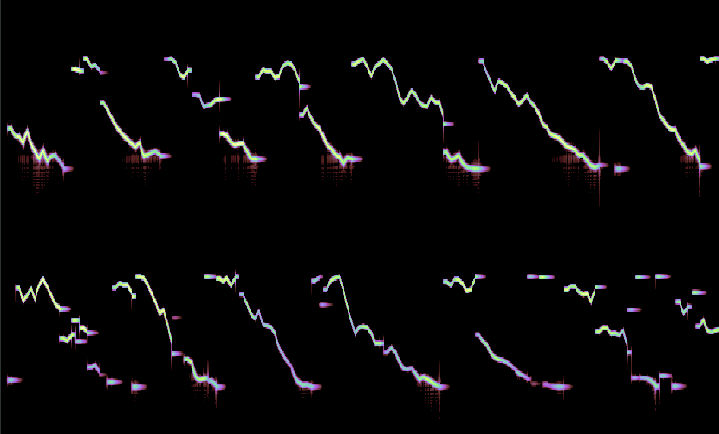
\includegraphics[width=\textwidth]{figures/sonif-3-bounce-sonogram.jpg}
\caption{Sonogram from the bounce of sonification-3. Time elapses from left-to-right (duration 30 seconds), frequencies from bottom-to-top (lowest excited frequency is 200 Hz, highest excited frequency is 4 kHz. Top half shows left channel, corresponding to too-hot anomalies. Bottom half shows right channel, corresponding to too-cold anomalies.}
\label{fig:sonif-3-bounce-sonogram}
\end{figure}

\begin{figure}
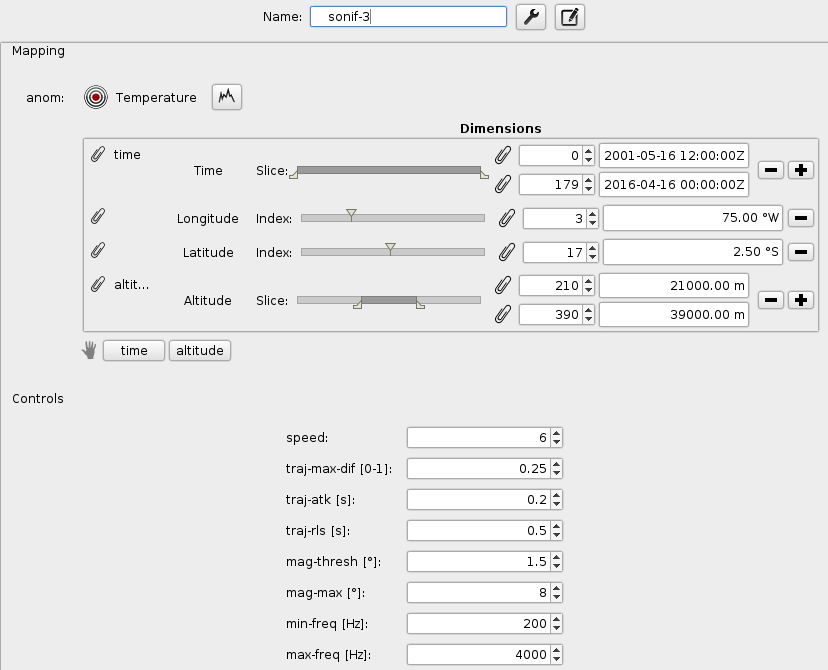
\includegraphics[width=\textwidth]{figures/sonif-3-editor-shot.jpg}
\caption{Matrix selection and parameter settings for sonification-3.}
\label{fig:sonif-3-editor-shot.jpg}
\end{figure}

% \printbibliography

\end{document}